\documentclass{tufte-handout}

\title{On ultimate; O2: secondary middle or popper}
\author[James Reynolds]{James Reynolds}

%\date{28 March 2010} % without \date command, current date is supplied

%\geometry{showframe} % display margins for debugging page layout

\usepackage{graphicx} % allow embedded images
  \setkeys{Gin}{width=\linewidth,totalheight=\textheight,keepaspectratio}
  \graphicspath{{graphics/}} % set of paths to search for images
\usepackage{amsmath}  % extended mathematics
\usepackage{booktabs} % book-quality tables
\usepackage{units}    % non-stacked fractions and better unit spacing
\usepackage{multicol} % multiple column layout facilities
\usepackage{lipsum}   % filler text
\usepackage{fancyvrb} % extended verbatim environments
  \fvset{fontsize=\normalsize}% default font size for fancy-verbatim environments

% Standardize command font styles and environments
\newcommand{\doccmd}[1]{\texttt{\textbackslash#1}}% command name -- adds backslash automatically
\newcommand{\docopt}[1]{\ensuremath{\langle}\textrm{\textit{#1}}\ensuremath{\rangle}}% optional command argument
\newcommand{\docarg}[1]{\textrm{\textit{#1}}}% (required) command argument
\newcommand{\docenv}[1]{\textsf{#1}}% environment name
\newcommand{\docpkg}[1]{\texttt{#1}}% package name
\newcommand{\doccls}[1]{\texttt{#1}}% document class name
\newcommand{\docclsopt}[1]{\texttt{#1}}% document class option name
\newenvironment{docspec}{\begin{quote}\noindent}{\end{quote}}% command specification environment

\begin{document}

\maketitle% this prints the handout title, author, and date
%\printclassoptions
This is 
a two-pager 
on being 
secondary middle/popper
on offence\footnote{
Referred to here 
as position O2.
This
is part of a series, 
available at
\url{https://github.com/James-Reynolds/Ultimate-strategy-and-tactics}}. 

\section{Beating person-match defence with a vertical stack}\label{sec:vertical}

\begin{marginfigure}%
  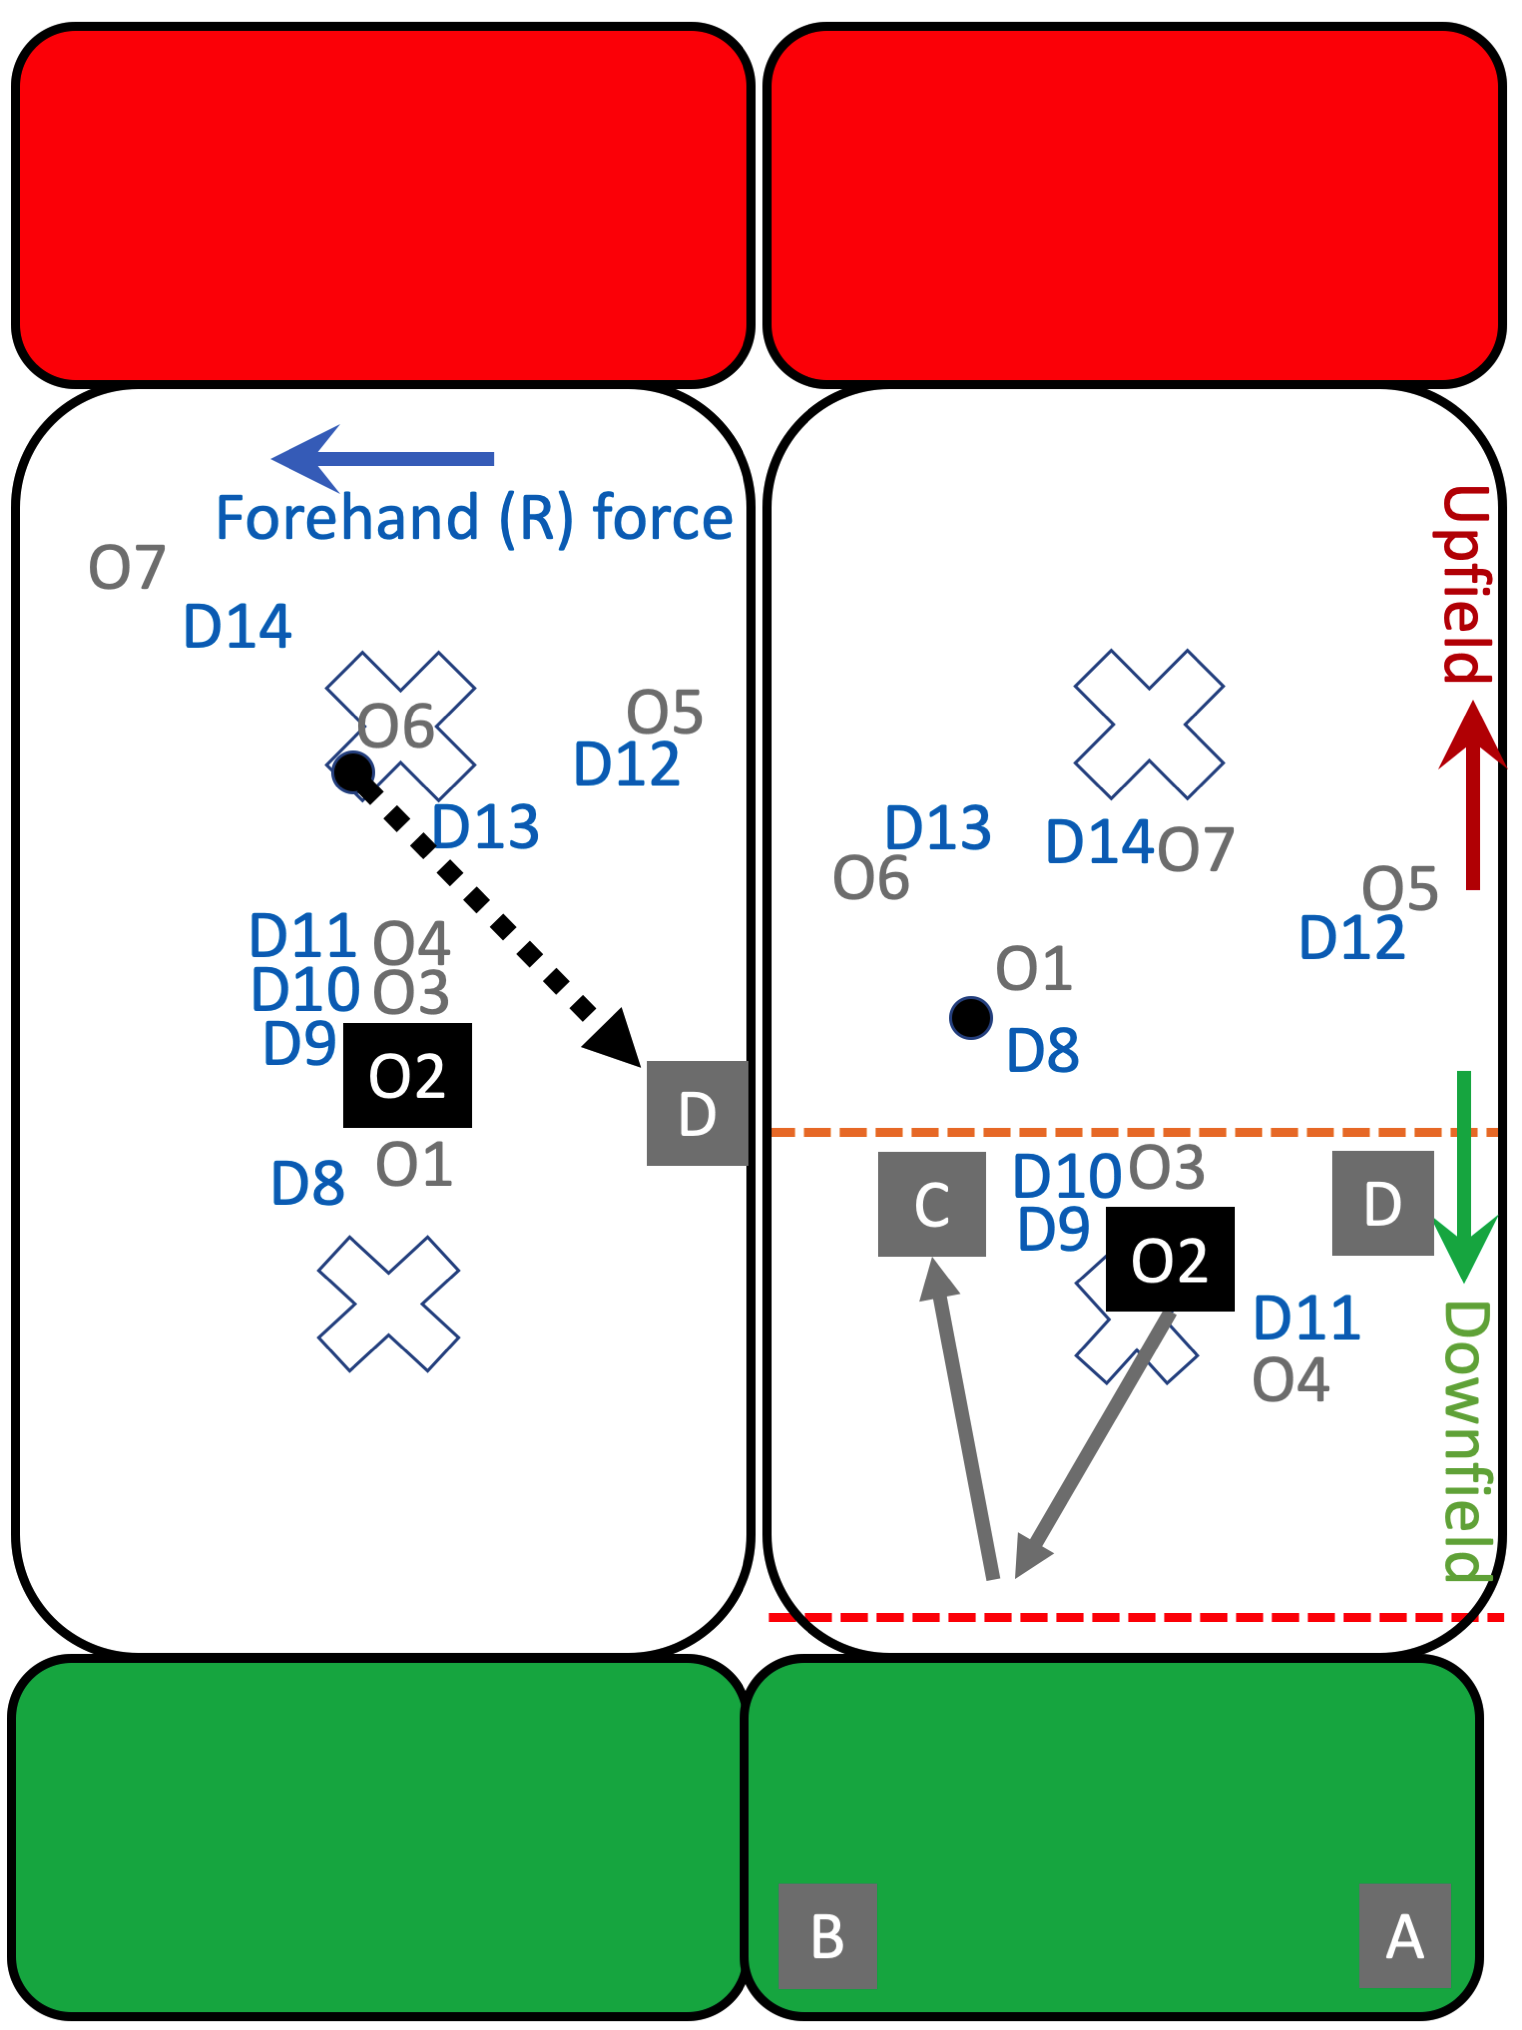
\includegraphics[width=\linewidth]{O2-vertical}
  \caption{Vertical stack: 
  starting position (left),
  and development (right)}
  \label{fig:O2-vertical}
\end{marginfigure}


Figure \ref{fig:O2-vertical} (left) shows 
a situation 
with 
your team: 
using 
a vertical stack formation; 
having called a brick; and
facing a 
forehand force with 
person-match defence\footnote{
Vertical works
against other person-match defences, 
but might need 
adjustment e.g. 
(1) backhand force,
mirror everything;
(2) straight up force, 
wait while handlers 
move it about 
until they can huck 
to you or O1;
(3) last-person-covers-deep,
coordinate with O1 
to overload D8 (deep) 
or D9 (under); etc.}. 
O6 is shown
potentially throwing 
a break throw to D 
(dashed black arrow).
You 
(O2)
or any of the other cutters
(O1. O3, O4) 
might run onto 
this pass 
after it is thrown\footnote{
Note, cutting to D 
before the throw 
risks causing a pick, 
as D9 
might be obstructed
 by O1 
 or O3. 
 However, 
 if you do not move 
 until the disc is in the air
 the pass may stand,
 with any pick 
 just allowing 
 D9 to
 catch up 
 to put the force on 
 a bit earlier.}.


Otherwise, 
as secondary middle, 
(O2) 
your role 
will likely 
involve cutting 
\smallcaps{after} 
the primary middle 
(O1)\footnote{
Starting
in the middle of the vertical stack,
as shown in 
Figure \ref{fig:O2-vertical} (left),
it is difficult for 
you to make 
an inital cut 
without causing 
a pick. 
In contrast, 
Figure \ref{fig:O2-vertical} (right)
shows O1 
having cut upfield 
and received 
a pass 
on the open side, 
which immediately 
frees you 
(O2) 
to cut 
from the back of the stack,
with less chance 
of a pick occurring.}.
The play might develop 
in lots of different ways, 
but
Figure \ref{fig:O2-vertical} (right) shows 
one outcome, 
with the disc going
to O1\footnote{
O1 has cut under 
on the open side.
O4 is indicated 
clearing 
or cutting 
deep on 
the break side. 
The stack is shown having 
moved further downfield.}. 
This leaves 
you 
available 
at the back of the stack. 
You might: 
(1) stand still until O1
(or someone else)  
throws it 
to A 
or D\footnote{
These throws  
break the force, 
so it is likely 
that D9 will 
be on the wrong side 
of you to make an interception.};
(2) cut to B, 
or (3) cut 
back under 
to C 
(grey arrows).  

O2 is called secondary middle, 
because you cut second, 
not because the position 
is of secondary importance. 
Hence, 
playing 
O2 is about 
waiting for a 
good time to cut,
and otherwise 
staying in the stack 
so that the defence 
always has to worry 
you receiving 
a throw to A. 
Too many cuts at once 
means you may 
get in each others way, 
and/or run out of people
in a good position 
to cut next.  

When cutting,
staying  
between 
the dashed 
horizontal 
lines 
may help. 
The position of 
the lines vary
with the position of the disc
and with how far the thrower  
can or will 
throw. 
However, 
if you go 
downfield of the dashed red line 
before the disc is in the air,
D9 (your marker) 
may be able 
get to
A or B 
before the disc,
intercepting 
or preventing 
any deep throws. 
Similarly, 
if you go 
upfield of the dashed yellow line
then D9 may 
be able to help
prevent dumps.

If you do get the disc,
look to immediately \smallcaps{make ground 
or throw a goal} 
to O1, 
O3 
or O4. 
However, 
you a cutter, 
so the most 
important things to do are:
to make sure your team 
retains possession of the disc; and
that you cut some more. 
Hence, 
if no pass downfield 
is immediately available, 
it is probably time to engage 
one of O5-7, 
throw a dump, 
and get downfield again 
(and into the stack).


\subsection{Beating person-match defence with feldrunner}
\label{sec:feld}
Figure \ref{fig:O2-horizontal} (left) 
shows a feldrunner formation, 
with 4 handlers (O4-7), 
and O1 as the focus.
You  
(O2) 
and O3
are in the endzone.

The idea of feldrunner 
is to pass to 
the isolated
focus (O1). 
They will then either pass to 
O3 or you, 
or dump to the handlers
and reset. This formation relies 
on you and O3 
waiting until O1 
gets the disc 
before making a cut.  
\begin{marginfigure}%
  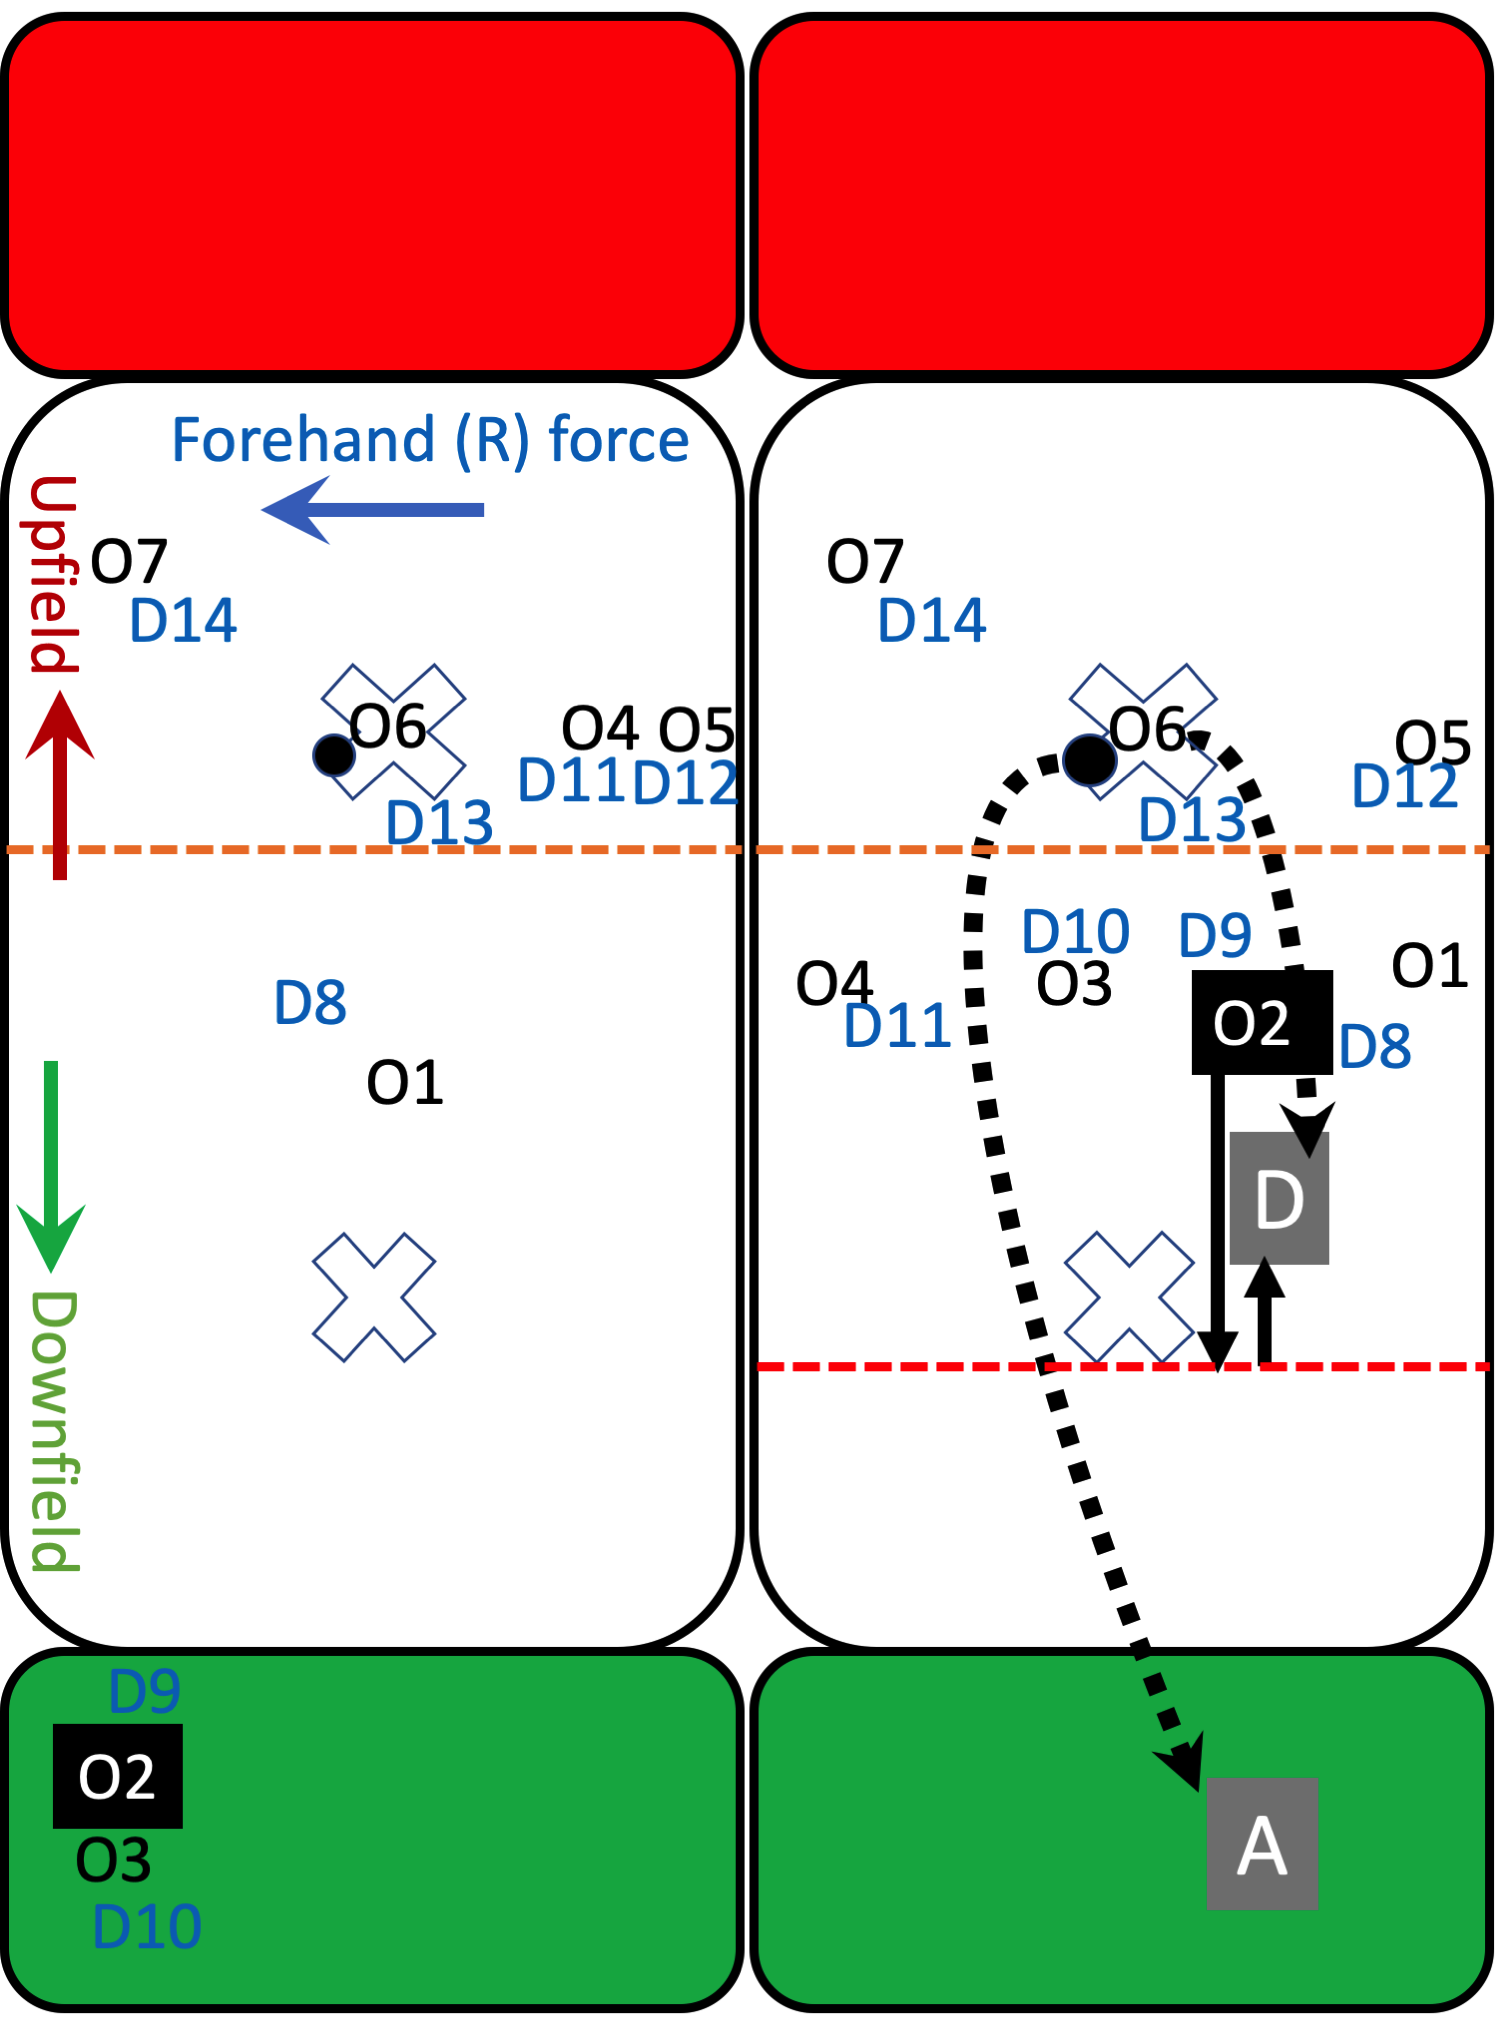
\includegraphics[width=\linewidth]{O2-horizontal}
  \caption{Feld (left) \& ho-ro (right)}
  \label{fig:O2-horizontal}
\end{marginfigure}

It may be that 
one of 
D9 
and D10 
go to help D8 
cover D1.  
If so, 
you and O3 
might spread out, 
one on each side line,
and move a bit closer, 
so as to receive a pass from 
the handlers directly.  


\subsection{Beating person-match defence with a horizontal stack}\label{sec:horizontall}
Horizontal stack 
typically involves cutting
upfield and downfield (black arrows)
within your quarter of the field\footnote{
Other cuts
can work, 
but might need
communication,
e.g. diamond cuts 
involve trading places 
with O1 
or O3.}
as shown in 
Figure \ref{fig:O2-horizontal}(right).
O6 
can potentially 
throw to you 
at A 
or D\footnote{
Black arrows
show how a back-under cut 
opens space 
for the throw 
to D.}. 

\section{Beating zone defence}\label{sec:zone}
\begin{marginfigure}%
  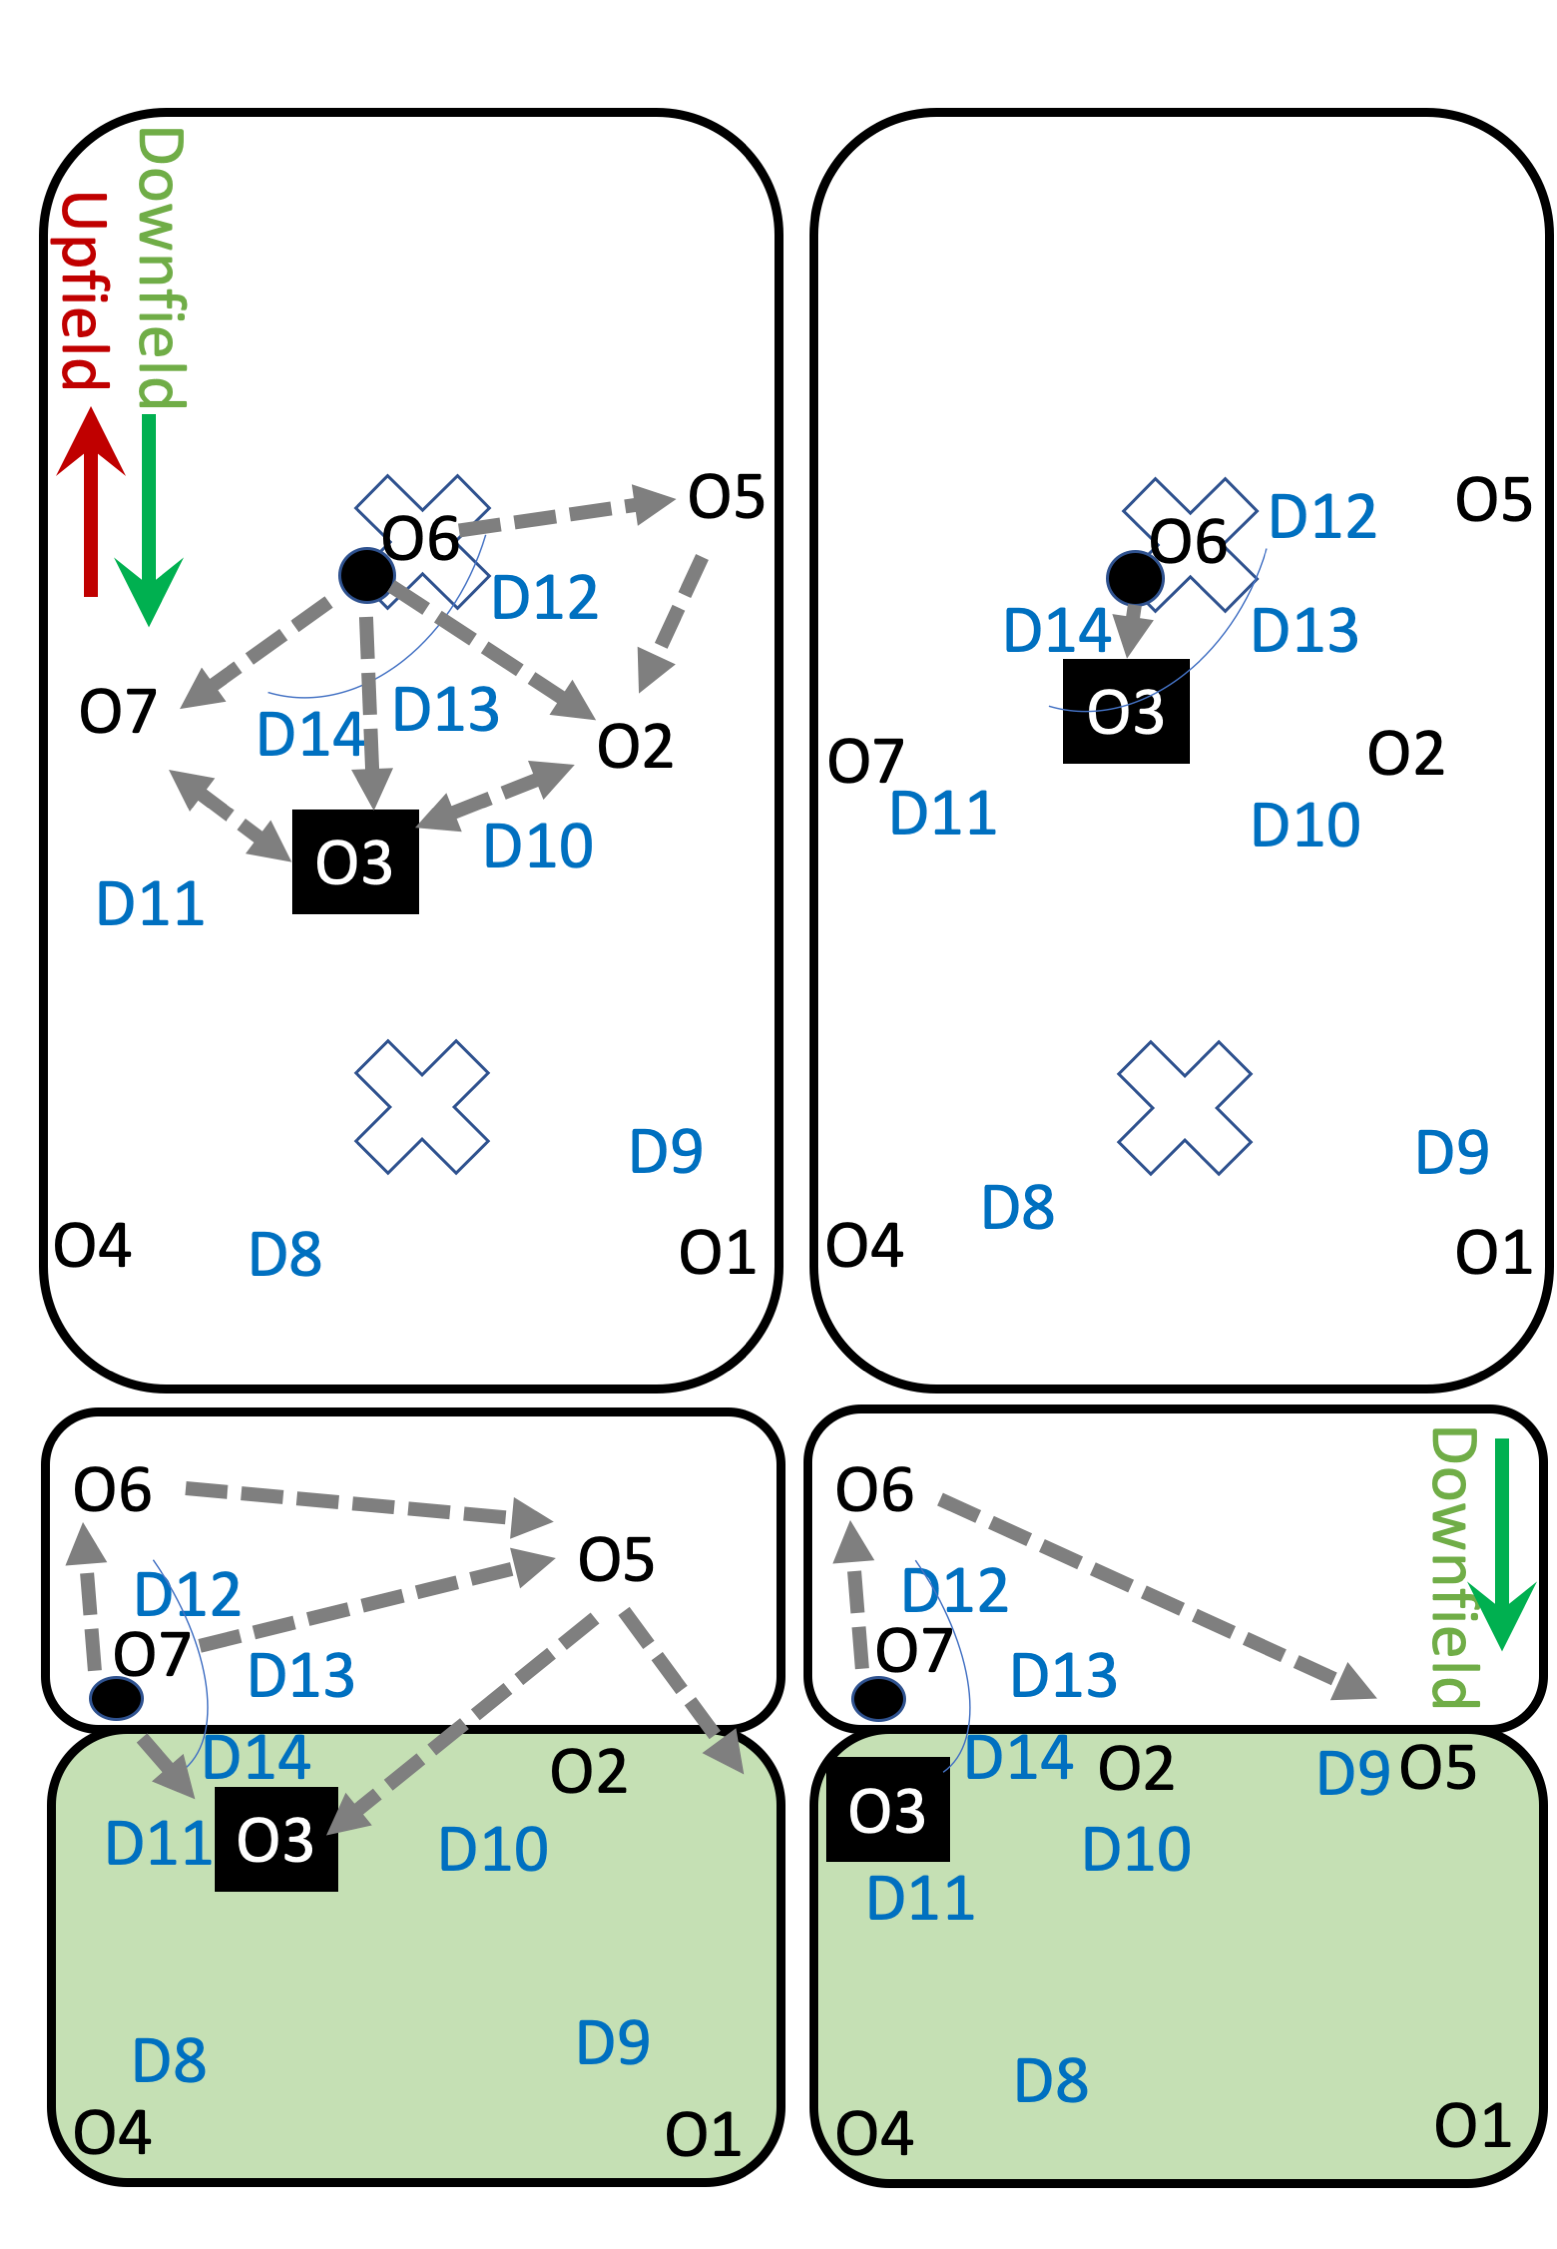
\includegraphics[width=\linewidth]{O2-zone331}
  \caption{formations against 331 zone}
  \label{fig:O2-zone331}
\end{marginfigure}
Vertical stack 
probably won't work
against zone. 
Instead, your 
team might do better spreading out, 
as shown 
in Figure \ref{fig:O2-zone331}. 

Three ways to beat a zone are:
(1) over;
(2) round; or
(3) through. 
Figure \ref{fig:O2-zone331}
(top left)
shows this 
with you 
behind the cup, 
potentially receiving a pass 
\smallcaps{through} 
the gap between 
D12 
and D13, or 
\smallcaps{over} 
the cup\footnote{
Short hammer, scoober.}.
Alternatively, 
it might go \smallcaps{round} 
with a pass to 
O5, 
who then 
throws to you.

An issue 
to keep in mind 
is how you 
coordinate 
with O3 
to split 
D10. 
Figure \ref{fig:O2-zone331}
(top left), 
shows D10 
having to 
cover both 
you and O3, 
with perhaps some help 
from D9 
and D11. 
In contrast, 
Figure \ref{fig:O2-zone331}
(top right) 
shows a position 
that might occur 
if you `crash' 
the cup\footnote{ 
Crashing 
might  
disrupt the 
cup's formation and 
allow a stall reset 
I'm not a huge fan, 
unless its a handlers 
crashing from behind, 
because you lose 
a player downfield},
which allows
D10 
to ignore you 
and play 
tighter on O3\footnote{ 
It might also allow 
D9 to threaten to intercept 
a pass to O5 
(blue arrow), 
and have further,
cascading, 
impacts. 
In general, 
by crashing the cup
from downfield 
the situation 
becomes 3 (O1, O3 and O4) 
versus 4 (D8-11) 
downfield of the cup, 
which is not ideal.}. 
An exception, 
however,
is shown in 
Figure \ref{fig:O2-zone331}
(bottom right)
where, close to the endzone, 
moving in towards 
the cup 
might suck D10 
in as well, 
opening more space for O5 
in the far front corner.  
Alternatively, 
Figure \ref{fig:O2-zone331}
(bottom left), 
indicates how spreading 
across the front of the endzone
might split D10, 
so 
from O5 
it can go to  
either you 
or O3. 


\section{Beating clam defence}\label{sec:zone}
Clam mixes person-match 
and zone defence styles, 
with defenders 
switching frequently
%\footnote{
%For example, 
%in Figure \ref{fig:O2-vertical}(left) 
%D8 
%might cover 
%O1 deep, 
%switching later 
%(with D9 or D11
%to cover O4's cut deep,
%rather than following O1 
%upfield to C.}. 
You might
coordinate 
with others  
to overload 
a defender, 
or spread out 
and give the handlers 
space 
and targets deep. 

\newthought{...and finally} 
this is just a two pager; 
there are many more 
offensive strategies 
and tactics\footnote{
Try Star Wars offence: 
No formation, but
Vader (O4), 
Palpatine (O3) and 
(Darth) Jar Jar (O1) can throw/receive amongst themselves;
same for Obi-Wan (O5), 
Luke (O1) 
and Leia (O2); 
Jar Jar 
and Obi-Wan 
can throw to each other. 
Yoda (O6) throws/receives to/from anyone;
No other throws allowed}.  
Remember, 
defence wins games, 
offence loses them\footnote{
Least turnovers 
usually wins.} 
and after a turnover 
it's better to get it back 
with another turnover, 
than receiving another pull!

\end{document}
